\begin{savequote}[8cm]
{\frakfamily
Daß ich erkenne, was die Welt \\
Im Innersten zusammenhält
}

So that I know what holds\\
the innermost world together
  \qauthor{--- Johann Wolfgang von Goethe \cite{goethe_faust}}
\end{savequote}

\chapter{\label{ch:1-intro}Introduction}
Particle creation by black holes \cite{Hawking:1975vcx}. Quantum gravity effects can be described by dimension-$6$ operators suppressed by the Planck scale $G_\text{Pl} ~ 10^{19}$ GeV \cite{IceCube:2021tdn}:
%
\begin{align} \label{eq:qg-operator}
    H \sim \frac{m^2}{2E} + \hat{a}^{(3)} - E \cdot \hat{c}^{(4)} + \hat{a}^{(5)} - E^3 \cdot \hat{c}^{(6)} ... \ \text{.}
\end{align}
%

\minitoc

First paper on gravitational effects in neutrino oscillations? \cite{Ahluwalia:1996ev}

\section{Motivation}
\cite{Kayser:2005cd}
\acrfull{dune}

relic neutrinos \cite{Aydiner:2022zcx}.

Unless otherwise stated, natural units $c=\hbar = 1$ are used in this thesis.

\section{\texorpdfstring{\acrlong{lbl}}{TEXT} Neutrino Oscillations}\label{subsec:lbl_osc}
%
%\ohead{\ref{subsec:lbl_osc} \ \acrshort{lbl} Neutrino Oscillation Experiments}
%
After a neutrino is produced in a flavour eigenstate, the propagating mass eigenstates experience different phase variations, leading  to the conversion of one flavour into another, which is referred to as the phenomenon of neutrino oscillations. The motivation of the project presented in this report is to carry out new \acrfull{bsm} physics searches with respect to neutrino oscillations in the \acrfull{t2k} and the next-generation long-baseline neutrino experiment \acrfull{dune}.
In the Standard Model of Particle Physics, the three generations (flavours) of neutrinos correspond to three weak interaction eigenstates $\ket{\nu_\alpha}$ of flavour $\alpha = \{\text{e},\mu,\tau\}$. As particles propagate in free space as eigenstates of the energy-momentum Hamiltonian, the basis of the weak interaction eigenstates can be related to the basis of mass propagation eigenstates $\ket{\nu_i}$ with $i=\{1,2,3\}$, each with mass $m_i$ by a unitary matrix. The most popular parametrisation of this unitary transformation matrix is the \acrfull{pmns} matrix given by $U_{\alpha i}$ \cite{Kayser:2005cd}:
\vspace{-2mm}%
%
\begin{align} \label{pmns}
\ket{\nu_\alpha} = \underline{\underline{U}}_{\alpha i} \ket{\nu_i} \quad \Leftrightarrow \quad \ket{\nu_i} =  U_{\alpha i}\ket{\nu_\alpha} \quad 
\text{with} \quad U_{\alpha i} =
\begin{pmatrix}
    U_{\text{e}1} & U_{\text{e}2} & U_{\text{e}3} \\
    U_{\mu 1} & U_{\mu 2} & U_{\mu 3} \\
    U_{\tau 1} & U_{\tau 2} & U_{\tau 3}
\end{pmatrix}
\end{align}
%
where $\ket{\nu_\alpha} =  U_{\alpha i}^*\ket{\nu_i}$.
%The flavor-$\alpha$ fractions of the mass eigenstates are shown in \Cref{fig:mass_hierarchy}.
The neutrino oscillation parameters are extracted via the neutrino oscillation probability. %The probability for a neutrino of mass eigenstate $\nu_i$ to produce a charged lepton of flavor $\alpha$ resulting from a \acrfull{cc} interaction in a detector is given by $|U_{\alpha i}|^2$.
The signal-only neutrino-event rate $R^\text{signal}_{\overset{\brobor}{\nu}_{\hspace{-1mm}\alpha} \rightarrow \overset{\brobor}{\nu}_{\hspace{-1mm}\beta}}$ for $\overset{\brobor}{\nu}_{\hspace{-1mm}\alpha} \hspace{-1mm} \rightarrow \hspace{-1mm} \overset{\brobor}{\nu}_{\hspace{-1mm}\beta}$ oscillations measurable in detectors is \cite{doi:10.1146/annurev-nucl-101917-020930}
%
%\begin{small}
\vspace{-3mm}
    \begin{align} \label{eq:nu_osc_prob}
        R^\text{signal}_{\overset{\brobor}{\nu}_{\hspace{-1mm}\alpha}\rightarrow\overset{\brobor}{\nu}_{\hspace{-1mm}\beta}}(p_\text{reco}) = \hspace{-1mm}\int\displaylimits_{E_\text{min}}^{E_\text{max}} \hspace{-1mm}\Phi_\alpha(E_\text{true}) \cdot \sum_{i,j} \sigma^i_\beta(E_\text{true}, p_\text{reco}) \cdot N_j \cdot \varepsilon_\beta(E_\text{true}, p_\text{reco}) \cdot P_{\overset{\brobor}{\nu}_{\hspace{-1mm}\alpha}\rightarrow\overset{\brobor}{\nu}_{\hspace{-1mm}\beta}}(E_\text{true}) \ ,
%       N_\text{det} = \Phi(E_\text{true}) \sigma(E_\text{true})    \varepsilon(E_\text{true},E_\text{rec}) P_\text{osc}
    \end{align}
%\end{small}
%\vspace{-2mm}%
where the event rate is a function of the reconstructed kinematic variables $p_\text{reco} \equiv (E_\text{reco}, \mathbf{p}_\text{reco})$, $\Phi_\alpha$ is the neutrino flux of flavor $\alpha$, $\sigma^i_\beta$ is the cross section for a neutrino $\nu_\beta$ of flavor $\beta$ with the target nucleus for interaction $i$, $N_j$ is the number of target nuclei in the detector fiducial volume of type $j$, $\varepsilon_\beta$ is the detector efficiency for flavor $\beta$ and $P_{\alpha\rightarrow\beta}$ is the neutrino oscillation probability for a neutrino to change from flavor $\alpha$ to flavor $\beta$. In order to extract the neutrino oscillation probability via \Cref{eq:nu_osc_prob}, oscillation experiments predict and measure %the neutrino flux in their near, pre-oscillation detectors and determine 
event rates using both near and far detectors. The near detector constrains the product of neutrino flux, cross section and detector response, which is then used to predict the event rate at the far detector, where oscillation effects are probed. 

Conversely using the same flux, cross section and detector property predictions, any deviation in the measured event rate at the far detector of an experiment from the expectation assuming the standard $3$$\times$$3$-\acrshort{pmns} formalism  might stem from an alternative neutrino oscillation probability and thus hints on new physics.

\section{State-of-the-Art of the Neutrino-Oscillation Landscape}
%{\color{red} Do I need an introduction to DUNE and T2K?}
The \acrfull{lbl} neutrino oscillation experiments \acrshort{dune} and \acrshort{t2k} aim to precisely measure the neutrino oscillation parameters, search for leptonic \acrshort{cp} violation, detect supernova-neutrinos and study neutrino interactions \cite{DUNE:2020ypp,T2K:2011qtm}. Mutual science goals in both experiments are complemented by ancillary programmes customised to the physics that either experiment is more sensitive to. \acrshort{dune} is proposed to leverage a wide-band neutrino beam in the $2$-$4$ GeV region operating on a $1300$ km baseline, whereas \acrshort{t2k}'s neutrinos have flux peak energies around $0.6$ GeV on a $295$ km baseline. The experimental baselines as well as muon-neutrino disappearance probabilities are visualised in \Cref{fig:exps_logos}.
%
\begin{figure}[H]
	%\begin{minipage}[b]{.47\textwidth}
	%\includegraphics[width=\textwidth]{figures/dune_lbl_logo}
    \begin{minipage}[b]{.46\textwidth}
    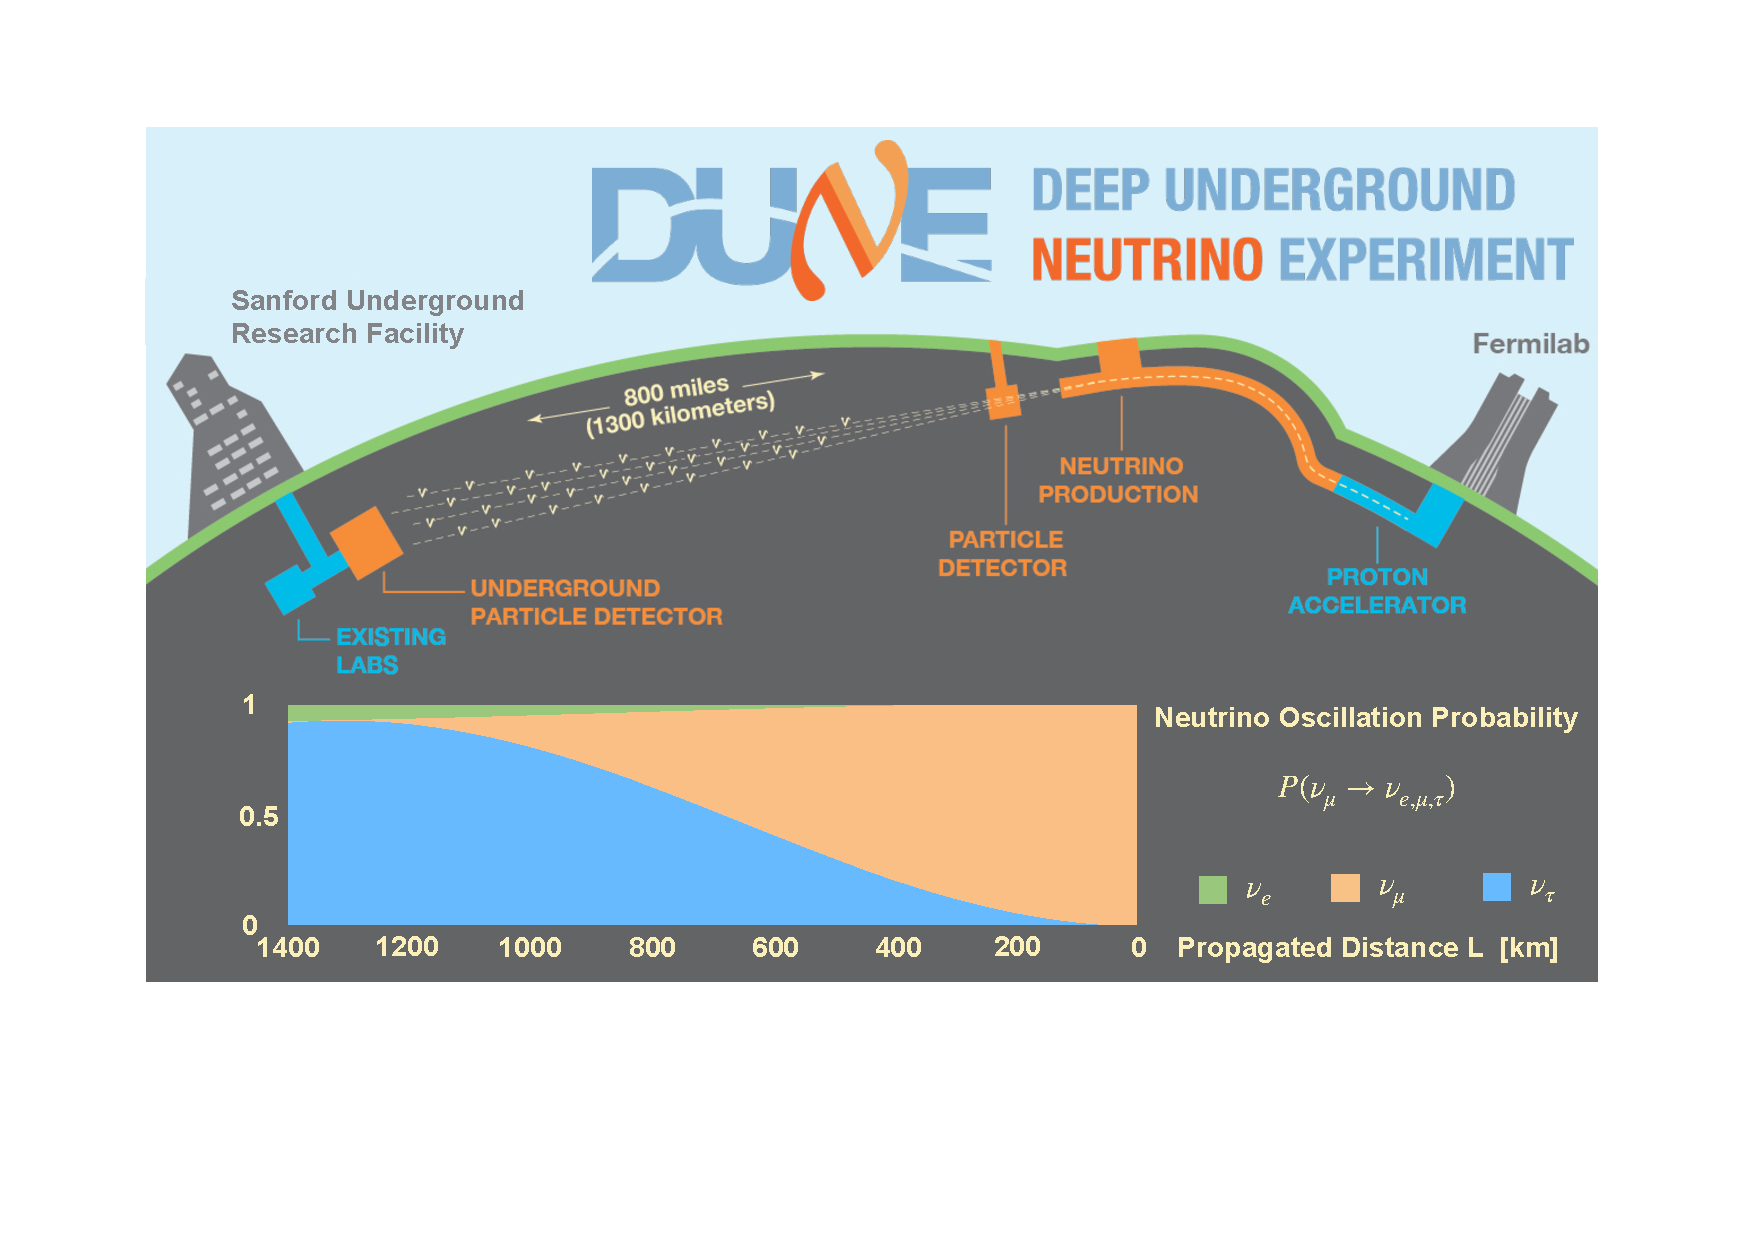
\includegraphics[width=\textwidth]{figures/intro/dune_lbl_logo_osc_prob}
	\end{minipage}
	%\begin{minipage}[b]{.51\textwidth}
	%\includegraphics[width=\textwidth]{figures/T2K_lbl_logo.pdf}
    \begin{minipage}[b]{.52\textwidth}
    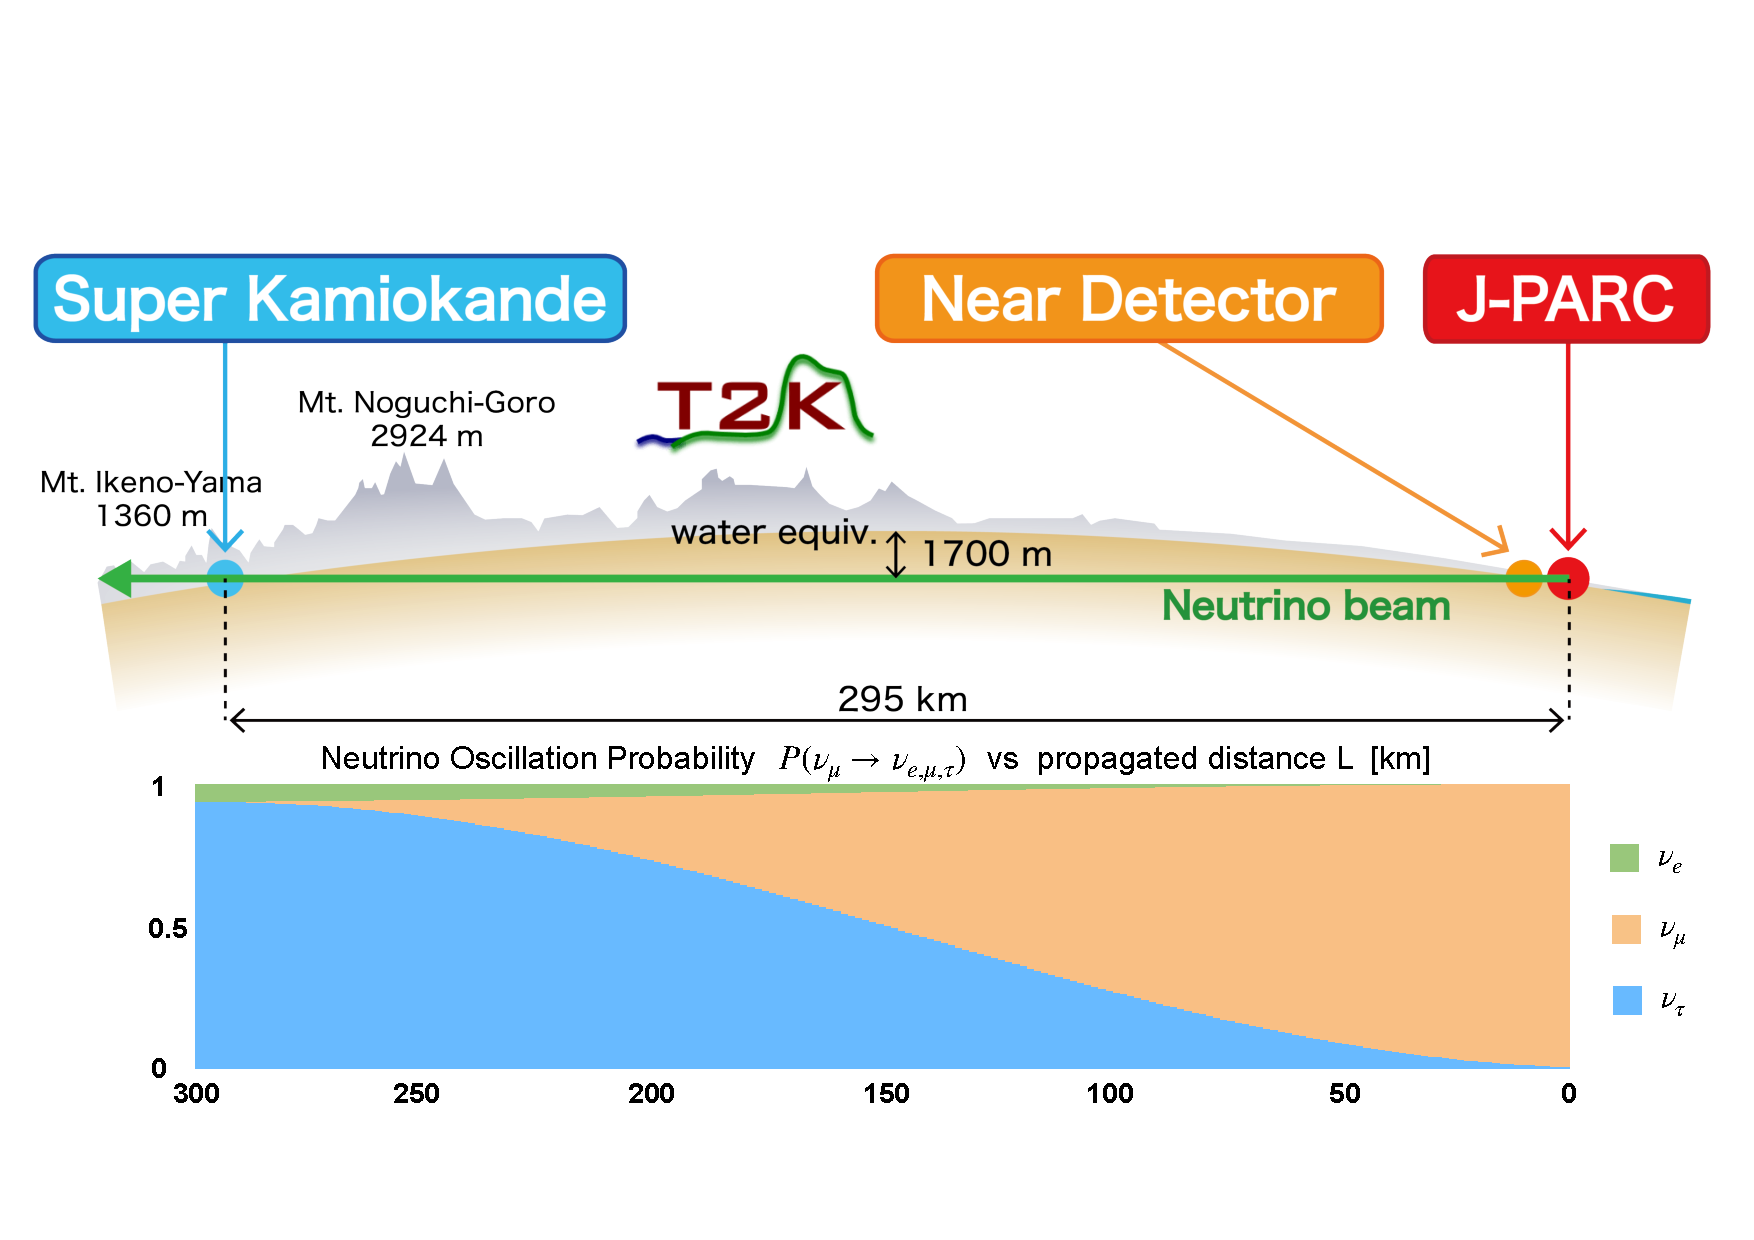
\includegraphics[width=\textwidth]{figures/intro/t2k_lbl_logo_osc_prob}
	\end{minipage}
	\caption{The long-baseline neutrino oscillation experiments \acrshort{dune} and \acrshort{t2k}. Left: Figure adapted from \cite{web:dune_lbl}. Right: Figure adapted from \cite{web:t2k_lbl}.}
	\label{fig:exps_logos}
\end{figure}
%
The different experimental setups allow complementary investigations of quantum decoherence in its many possible manifestations. Quantum decoherence is a phenomenon that might stem from various physical occurrences in nature \cite{Farzan:2008zv}. The formalism described in this report outlines and analyses different ways in which quantum decoherence could manifest as modifications to standard neutrino oscillations. Quantum gravitational effects are expected to make spacetime fluctuate at microscopic length or high-energy scales, making it a stochastic medium for neutrino propagation. Such stochastic perturbations may, for example, result from neutrino-virtual black hole interaction scenarios. The coupling of neutrinos to these effects could cause a phase shift of neutrino waves and give rise to decoherence and damping of neutrino oscillations over distance. On the other hand, the same effect on the neutrino oscillation probability could be caused by an anti-proportionality relation of the decoherence strength with respect to energy. This may be the case for a scenario in which lightcone fluctuations give rise to a neutrino experiencing distortions on its path through spacetime \cite{Stuttard:2021uyw}. My project is to investigate  quantum decoherence signatures in neutrino oscillations and determine the sensitivity for measurements in \acrshort{dune} and \acrshort{t2k}.

\subsection{The T2K Experiment}

\subsection{The DUNE Experiment}
The DUNE experiment is a $1300$km long-baseline neutrino oscillation experiment with the goal of measuring neutrino oscillation parameters, searching for CP violation, proton decay and supernova neutrinos. Moreover, there is a physics program for beyond the standard model physics, atmospheric neutrinos, dark matter searches as well as a rich neutrino interaction program. One of the roles of the DUNE near detector is the tuning of the neutrino-nucleus interaction model.

\section{Neutrino Interactions with Matter}

\section{New Physics Searches - Quantum Decoherence}\label{subsec:decoh}
Alongside a non-exhaustive list of possible studies to search for new \acrfull{bsm} phyiscs, quantum decoherence has gained an increased popularity in recent years. Quantum Decoherence is a phenomenon that may stem from very differently motivated physical models (see a clearer outline of why this is in \Cref{subsec:oqsf}) and hence enables phenomenological studies covering a wide range of new physics prospects. Besides numerous existing phenomenological studies on quantum decoherence effects in neutrino oscillations \cite{DeRomeri:2023dht,Barenboim:2024wdn,Gomes:2020muc} and existing upper limits and sensitivity studies in the IceCube Neutrino Observatory \cite{IceCube:2021tdn,ICECUBE:2023gdv} and \acrfull{km3net} neutrino observatories \cite{KM3NeT:2024jji}, this study presents the first experimental analysis for quantum decoherence with accelerator-born neutrinos, in particular from the \acrshort{t2k} and \acrshort{dune} experiment. If we consider neutrino oscillations as the quantum superposition of neutrino mass eigenstates and decoherence as the loss of coherence, then decoherence in the context of neutrino oscillations means that there is no sustained mixing of neutrino mass eigenstates. This decoherence effect is fundamentally different from wave-packet decoherence\footnote{Wave-packet decoherence is produced via the separation of the neutrino mass states over long distances due to their differing masses.} in the sense that it is induced by the environment that the neutrino propagates through rather than by the dispersion of wave packets.